\documentclass[12pt, oneside]{article}

\usepackage[letterpaper, scale=0.89, centering]{geometry}
\usepackage{fancyhdr}
\setlength{\parindent}{0em}
\setlength{\parskip}{1em}

\usepackage{tikz}
\usetikzlibrary{automata,positioning,arrows}

\pagestyle{fancy}
\fancyhf{}
\renewcommand{\headrulewidth}{0pt}
\rfoot{\href{https://creativecommons.org/licenses/by-nc-sa/2.0/}{CC BY-NC-SA 2.0} Version \today~(\thepage)}

\usepackage{amssymb,amsmath,pifont,amsfonts,comment,enumerate,enumitem}
\usepackage{currfile,xstring,hyperref,tabularx,graphicx,wasysym}
\usepackage[labelformat=empty]{caption}
\usepackage{xcolor}
\usepackage{multicol,multirow,array,listings,tabularx,lastpage,textcomp,booktabs}

\lstnewenvironment{algorithm}[1][] {   
    \lstset{ mathescape=true,
        frame=tB,
        numbers=left, 
        numberstyle=\tiny,
        basicstyle=\rmfamily\scriptsize, 
        keywordstyle=\color{black}\bfseries,
        keywords={,procedure, div, for, to, input, output, return, datatype, function, in, if, else, foreach, while, begin, end, }
        numbers=left,
        xleftmargin=.04\textwidth,
        #1
    }
}
{}

\newcommand\abs[1]{\lvert~#1~\rvert}
\newcommand{\st}{\mid}

\newcommand{\cmark}{\ding{51}}
\newcommand{\xmark}{\ding{55}}
 
\begin{document}
\begin{flushright}
    \StrBefore{\currfilename}{.}
\end{flushright} 
\subsection*{Week 2 at a glance}

\vspace{-15pt}

\subsubsection*{Textbook reading: Sections 1.1, 1.2}

\vspace{-15pt}

Before Monday, read Figure 1.4 and Definition 1.5 (definition of finite automata) on pages 34-35.

Before Wednesday, read pages 41-43 (Figures 1.18, 1.19, 1.20) for examples of automata and languages. Wednesday's class will be asynchronous. Please read over the annotated notes and watch the relevant supplementary videos. Ask any followup questions in the discussion forum or in office hours.

Before Friday, read pages 48-50 (Figures 1.27, 1.29) which introduces nondeterminism.

No class on Week 3 Monday in observance of Martin Luther King Jr. Day.

For Week 3 Wednesday: read the definition of the union, concatenation, and star operations for languages,  given 
as Definition 1.23 on page 44 and a useful example is Example 1.24.

\vspace{-20pt}

\subsubsection*{We will be learning and practicing to:}
\begin{itemize}
\item Clearly and unambiguously communicate computational ideas using appropriate formalism. Translate across levels of abstraction.
\begin{itemize}
   \item Give examples of sets that are regular (and prove that they are).
   \begin{itemize}
      \item {\bf State the definition of the class of regular languages}
      \item {\bf Give examples of regular languages, using each of the three equivalent models of computation for proving regularity.}
   \end{itemize}
   \item Describe and use models of computation that don't involve state machines.
   \begin{itemize}
      \item {\bf Given a DFA, find a regular expression that describes its language.}
      \item {\bf Given a regular expression, find a DFA that recognizes its language.}
   \end{itemize}
   \item Use precise notation to formally define the state diagram of finite automata.
   \item Use clear English to describe computations of finite automata informally.
      \begin{itemize}
         \item {\bf State the formal definition of (deterministic) finite automata}   
         \item {\bf Trace the computation of a finite automaton on a given string using its state diagram}
         \item {\bf Translate between a state diagram and a formal definition}
         \item {\bf Determine if a given string is in the language recognized by a finite automaton}
         \item {\bf Design an automaton that recognizes a given language}
         \item {\bf Specify a general construction for DFA based on parameters}
         \item {\bf Design general constructions for DFA}
   \end{itemize}
\end{itemize}

\end{itemize}

\vspace{-50pt}

\subsubsection*{TODO:}
\begin{list}{\itemsep-10pt}
   \item \#FinAid Assignment on Canvas (complete as soon as possible) and read syllabus on Canvas
   \item Schedule your Test 1 Attempt 1, Test 2 Attempt 1, Test 1 Attempt 2, and Test 2 Attempt 2 times 
   at PrairieTest (http://us.prairietest.com)
   \item Review Quiz 1 on PrairieLearn (http://us.prairielearn.com), complete by 1/15/25
   \item Review Quiz 2 on PrairieLearn (http://us.prairielearn.com), complete by 1/15/25
   \item Create a homework group, possibly by using the Piazza (https://piazza.com/) find-a-teammate tool
   \item Homework 1 submitted via Gradescope (https://www.gradescope.com/), due 1/16/25
\end{list}


\newpage

\subsection*{Week 2 Monday: Finite automata}




**This definition was in the pre-class reading**
A finite automaton (FA) is specified by  $M = (Q, \Sigma, \delta, q_0, F)$.
This $5$-tuple is called the {\bf formal definition} of the FA. The FA can also 
be represented by its state diagram: with nodes for the state, labelled edges specifying the 
transition function, and decorations on nodes denoting the start and accept states.

\begin{quote}
Finite set of states $Q$ can be labelled by any collection of distinct names. Often
we use default state labels $q0, q1, \ldots$ 
\end{quote}

\begin{quote}  
The alphabet $\Sigma$ determines the possible inputs to the automaton. 
Each input to the automaton is a string over  $\Sigma$, and the automaton ``processes'' the input
one symbol (or character) at a time.
\end{quote}

\begin{quote}
The transition function $\delta$ gives the next state of the automaton based on the current state of 
the machine and on the next input symbol.
\end{quote}

\begin{quote}
The start state $q_0$ is an element of $Q$.  Each computation of the machine starts at the  start  state.
\end{quote}

\begin{quote}
The accept (final) states $F$ form a subset of the states of the automaton, $F \subseteq  Q$. 
These states are used to flag if the machine accepts or rejects an input string.
\end{quote}


\begin{quote}
The computation of a machine on an input string is a sequence of states
in the machine,  starting with the start state, determined by transitions 
of the machine as it reads successive input symbols.
\end{quote}

\begin{quote}
The finite automaton $M$ accepts the given input string exactly when the computation of $M$ on the input string
ends in an accept state. $M$ rejects the given input string exactly when the computation of 
$M$ on the input string ends in a nonaccept state, that is, a state that is not in $F$.
\end{quote}

\begin{quote} 
The language of $M$, $L(M)$, is defined as the set of  all strings that are each accepted 
by the machine $M$. Each string that is rejected by $M$ is not in $L(M)$.
The language of $M$ is also called the language recognized by $M$.
\end{quote}   
   
What is {\bf finite} about all finite automata? (Select all that apply)
\begin{itemize}
   \item[$\square$] The size of the machine (number of states, number of arrows)
   \item[$\square$] The length of each computation of the machine
   \item[$\square$] The number of strings that are accepted by the machine
\end{itemize}
\newpage
  
\begin{center}
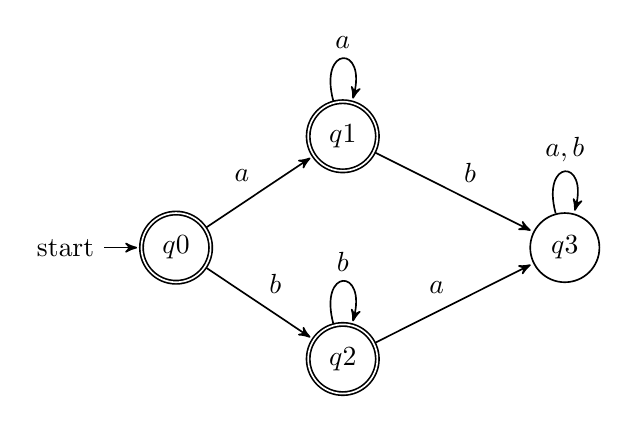
\begin{tikzpicture}[->,>=stealth',shorten >=1pt, auto, node distance=2cm, semithick]
   \tikzstyle{every state}=[text=black, fill=none]
   
   \node[initial,state,accepting] (q0)          {$q0$};
   \node[state,accepting]         (q1) [above right of=q0, xshift=20pt] {$q1$};
   \node[state,accepting]         (q2) [below right of=q0, xshift=20pt] {$q2$};
   \node[state]                   (q3) [below right of=q1, xshift=40pt] {$q3$};
   
   \path (q0) edge  [bend left=0] node {$a$} (q1)
       (q1) edge [loop above] node {$a$} (q1)
       (q1) edge [bend left=0] node {$b$} (q3)
       (q0) edge [bend left=0] node {$b$} (q2)
       (q2) edge [loop above] node {$b$} (q2)
       (q2) edge [bend left=0] node {$a$} (q3)
       (q3) edge [loop above] node {$a,b$} (q3)
   ;
\end{tikzpicture}
\end{center}
The formal definition of this FA is
   
\vfill
\vfill
   

Classify each string $a, aa, ab, ba, bb, \varepsilon$ as accepted by the FA or rejected by the FA.  

{\it Why are these the only two options?}

\vspace{200pt}


The language recognized by this automaton is
  

\vfill

\newpage

\begin{center}
   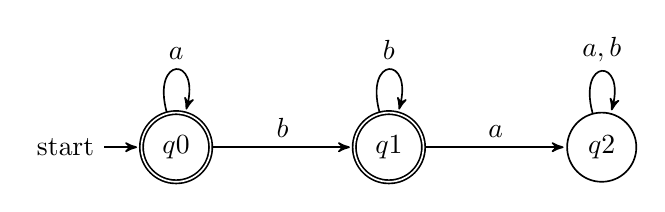
\begin{tikzpicture}[->,>=stealth',shorten >=1pt, auto, node distance=2cm, semithick]
      \tikzstyle{every state}=[text=black, fill=none]
      
      \node[initial,state,accepting] (q0)          {$q0$};
      \node[state,accepting]         (q1) [right of=q0, xshift=20pt] {$q1$};
      \node[state]         (q2) [right of=q1, xshift=20pt] {$q2$};
      
      \path (q0) edge  [bend left=0] node {$b$} (q1)
          (q0) edge [loop above] node {$a$} (q0)
          (q1) edge [bend left=0] node {$a$} (q2)
          (q1) edge [loop above] node {$b$} (q1)
          (q2) edge [loop above] node {$a,b$} (q2)
      ;
   \end{tikzpicture}
\end{center}

The language recognized by this automaton is
  


\vfill

\hrule

\begin{center}
   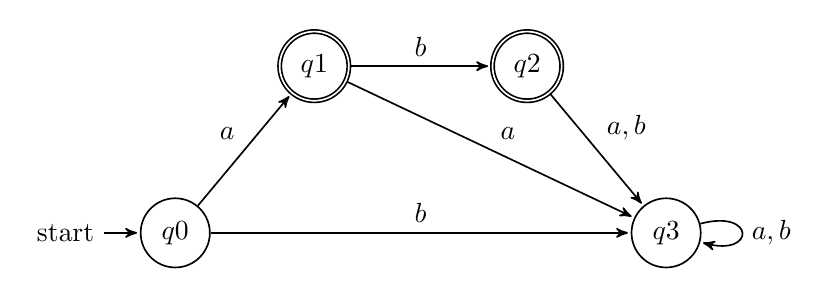
\begin{tikzpicture}[->,>=stealth',shorten >=1pt, auto, node distance=2cm, semithick]
      \tikzstyle{every state}=[text=black, fill=none]
      
      \node[initial,state] (q0)          {$q0$};
      \node[state,accepting]         (q1) [above right of=q0, xshift=10pt, yshift=20pt] {$q1$};
      \node[state,accepting]         (q2) [right of=q1, xshift=20pt] {$q2$};
      \node[state]          (q3) [below right of=q2, xshift=10pt, yshift=-20pt] {$q3$};
      
      \path (q0) edge  [bend left=0] node {$a$} (q1)
          (q0) edge [bend left=0] node {$b$} (q3)
          (q1) edge [bend left=0] node {$b$} (q2)
          (q1) edge [bend left=0] node {$a$} (q3)
          (q2) edge [bend left=0] node {$a,b$} (q3)
          (q3) edge [loop right] node {$a,b$} (q3)
      ;
   \end{tikzpicture}
\end{center}

The language recognized by this automaton is
  

\vfill 

\subsection*{Week 2 Wednesay: Finite automaton constructions - asynchronous}



{\bf Review}: Formal definition of DFA: $M = (Q, \Sigma, \delta, q_0, F)$ 

\begin{center}
\begin{multicols}{2}
\begin{itemize}
\setlength{\itemsep}{2pt}
\item Finite set of states $Q$
\item Alphabet $\Sigma$
\item Transition function $\delta$
\item Start state $q_0$
\item Accept (final) states $F$
\end{itemize}
\end{multicols}
\end{center}
Quick check: In the state diagram of $M$, how many outgoing arrows are there from each state?



{\bf Note}: We'll see a new kind of finite automaton. It will be helpful to distinguish it from the
machines we've been talking about so we'll use {\bf Deterministic Finite Automaton} (DFA) to refer to the machines 
from Section 1.1.

$M = ( \{ q0, q1, q2\}, \{a,b\}, \delta, q0, \{q0\} )$ 
where $\delta$ is  (rows labelled by states
and columns labelled by symbols):
\begin{center}
\begin{tabular}{c|cc}
$\delta$ & $a$ & $b$ \\
\hline
$q0$ & $q1$ & $q1$ \\
$q1$ & $q2$ & $q2$ \\
$q2$ & $q0$ & $q0$ \\
\end{tabular}
\end{center}

The state diagram for $M$ is 

\vfill


Give two examples of strings that are accepted by $M$ and two examples of strings that are rejected by $M$:

\vfill


A regular expression describing $L(M)$ is


\vfill 

A state diagram for a finite automaton recognizing
$$\{w \mid w~\text{is a string over $\{a,b\}$ whose length is not a multiple of $3$} \}$$

\vfill

Extra example: Let $n$ be an arbitrary positive integer. What is a formal definition for a finite automaton recognizing
\[
\{w \mid w~\text{is a string over $\{0,1\}$ whose length is not a multiple of $n$} \}?
\]

\newpage

Consider the alphabet $\Sigma_1 = \{0,1\}$.

A state diagram for a finite automaton that recognizes $\{w \mid w~\text{contains at most two $1$'s} \}$ is

\vfill
A state diagram for a finite automaton that recognizes $\{w \mid w~\text{contains more than two $1$'s} \}$ is

\vfill

\textbf{Strategy}: Add ``labels" for states in the state diagram, 
e.g. ``have not seen any of desired pattern yet'' or
``sink state''. Then, we can use the analysis of the roles of the states in the 
state diagram to work towards a description of the language recognized
by the finite automaton.


\vfill
\newpage
Or: decompose the language to a simpler one 
that we already know how to recognize with a DFA or NFA.


Textbook Exercise 1.14: 
Suppose $A$ is a language over an alphabet $\Sigma$. 
If there is a DFA $M$ such that $L(M) = A$ then there is another DFA, let's call it $M'$, such that 
$L(M') = \overline{A}$, the complement of $A$, defined as $\{ w \in \Sigma^* \mid w \notin A \}$.


{\bf Proof idea}:


\vfill
A useful bit of terminology: the {\bf iterated transition function} of a finite automaton
$M = (Q, \Sigma, \delta, q_0, F)$ is defined recursively by
\[
\delta^* (~(q,w)~) 
=\begin{cases}
q  \qquad &\text{if $q \in Q, w = \varepsilon$} \\
\delta( ~(q,a)~) \qquad &\text{if $q \in Q$, $w = a \in \Sigma$ } \\
\delta(~(\delta^*(~(q,u)~), a) ~) \qquad &\text{if $q \in Q$, $w = ua$ where $u \in  \Sigma^*$ and $a \in \Sigma$}
\end{cases}
\]

Using  this terminology, $M$ accepts a string $w$ over $\Sigma$ if and only if $\delta^*( ~(q_0,w)~) \in F$.


{\bf Proof}: 
\vfill

 
\newpage
\subsection*{Week 2 Friday: Nondeterministic automata}

We saw that whenever a language is recognized by a DFA, its
complement is also recognized by some (other) DFA. 

Another way to say this is that the collection of languages
that are each recognizable by a DFA is {\bf closed} under complementation.


Before we continue with more complicated constructions, let's revisit some of 
the assumption of the {\bf D}FA model.

Recall that the computation of {\bf deterministic} finite automaton has exactly one choice for its next step given the current state and the current character to read.




\begin{center}
\begin{tabular}{|ll|}
\hline
\multicolumn{2}{|l|}{{\bf Nondeterministic finite automaton}  (Sipser Page 53) Given as $M = (Q, \Sigma, \delta, q_0, F)$}\\
& \\
Finite set of states $Q$  & Can  be labelled by any collection  of distinct names. Default: $q0, q1, \ldots$  \\
Alphabet $\Sigma$ &  Each input to the automaton is a string over  $\Sigma$. \\
Arrow labels $\Sigma_\varepsilon$ &  $\Sigma_\varepsilon = \Sigma \cup \{ \varepsilon\}$. \\
&  Arrows 
in the state diagram are labelled either by symbols from $\Sigma$ or by $\varepsilon$ \\
Transition function $\delta$  & $\delta: Q \times \Sigma_{\varepsilon} \to \mathcal{P}(Q)$
gives the {\bf set of possible next states} for a transition \\
&  from the current state upon reading a symbol or spontaneously moving.\\
Start state $q_0$ & Element of $Q$.  Each computation of the machine starts at the  start  state.\\
Accept (final) states $F$ & $F \subseteq  Q$.\\
& \\
\multicolumn{2}{|p{\textwidth}|}{$M$ accepts the input string $w \in \Sigma^*$ if and only if {\bf there is} a computation of $M$ on 
$w$ that processes the whole string and ends in an
accept state.}\\
\hline
\end{tabular}
\end{center}

The formal definition of the NFA over $\{0,1\}$ given by this state diagram is: 

\begin{center}
    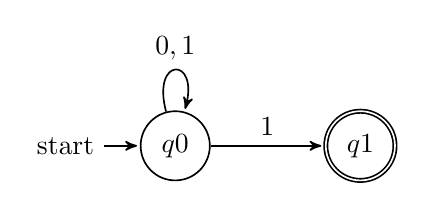
\begin{tikzpicture}[->,>=stealth',shorten >=1pt, auto, node distance=2cm, semithick]
       \tikzstyle{every state}=[text=black, fill=none]
       
       \node[initial,state] (q0)          {$q0$};
       \node[state,accepting]         (q1) [right of=q0, xshift=10pt]{$q1$};
       
       \path (q0) edge  [loop above] node {$0,1$} (q0)
           (q0) edge [bend left=0] node {$1$} (q1)
       ;
    \end{tikzpicture}
 \end{center}


The language over $\{0,1\}$ recognized by this NFA is:

\vspace{70pt}

{\it Practice}: Change the transition function to get a different NFA which accepts
the empty string (and potentially other strings too).


\newpage

The state diagram of an NFA over $\{a,b\}$ is:

\begin{center}
    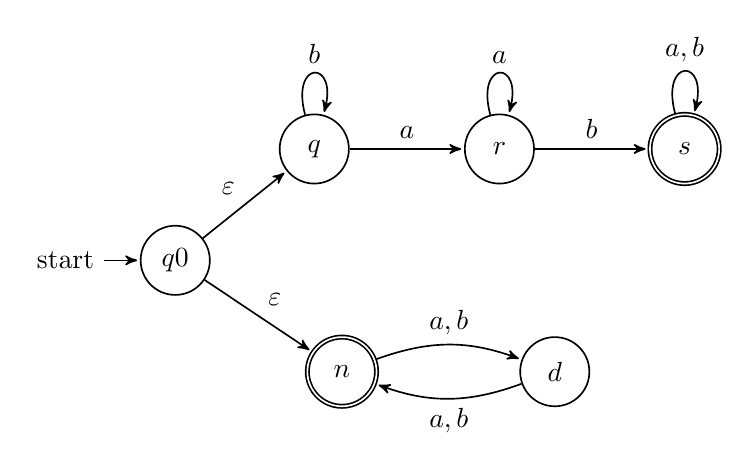
\begin{tikzpicture}[->,>=stealth',shorten >=1pt, auto, node distance=2cm, semithick]
       \tikzstyle{every state}=[text=black, fill=none]
       
       \node[initial,state] (q0)          {$q0$};
       \node[state,accepting]         (n) [below right of=q0, xshift=20pt] {$n$};
       \node[state]     (d) [right of=n, xshift=20pt] {$d$};
       \node[state]     (q) [above right of=q0, xshift=10pt] {$q$};
       \node[state]     (r) [right of=q, xshift=10pt] {$r$};
       \node[state,accepting]     (s) [right of=r, xshift=10pt] {$s$};
       
       \path (q0) edge  [bend left=0] node {$\varepsilon$} (q)
           (q0) edge  [bend left=0] node {$\varepsilon$} (n)
           (q) edge [bend left=0] node {$a$} (r)
           (q) edge [loop above] node {$b$} (q)
           (r) edge [bend left=0] node {$b$} (s)
           (r) edge [loop above] node {$a$} (r)
           (s) edge [loop above] node {$a,b$} (s)
           (n) edge [bend left=20] node {$a,b$} (d)
           (d) edge [bend left=20] node {$a,b$} (n)
       ;
    \end{tikzpicture}
 \end{center}

 The formal definition of this NFA is:

 \vfill

\newpage

Suppose $A_1, A_2$ are languages over an alphabet $\Sigma$.
{\bf Claim:} if there is a NFA $N_1$ such that $L(N_1) = A_1$ and 
NFA $N_2$ such that $L(N_2) = A_2$, then there is another NFA, let's call it $N$, such that 
$L(N) = A_1 \cup A_2$.

{\bf Proof idea}: Use nondeterminism to choose which of $N_1$, $N_2$ to run.

\vfill
\begin{comment}
    Draw schematic
\end{comment}

{\bf Formal construction}: Let 
$N_1 = (Q_1, \Sigma, \delta_1, q_1, F_1)$ and $N_2 = (Q_2, \Sigma, \delta_2,q_2, F_2)$
and assume $Q_1 \cap Q_2 = \emptyset$ and that $q_0 \notin Q_1 \cup Q_2$.
Construct $N = (Q, \Sigma, \delta, q_0, F_1 \cup F_2)$ where
\begin{itemize}
    \item $Q = $
    \item $\delta: Q \times \Sigma_\varepsilon \to \mathcal{P}(Q)$ is defined by, for $q \in Q$ and $x \in \Sigma_{\varepsilon}$:
        \[
            \phantom{\delta((q,x))=\begin{cases}  \delta_1 ((q,x)) &\qquad\text{if } q\in Q_1 \\ \delta_2 ((q,x)) &\qquad\text{if } q\in Q_2 \\ \{q1,q2\} &\qquad\text{if } q = q_0, x = \varepsilon \\ \emptyset\text{if } q= q_0, x \neq \varepsilon \end{cases}}
        \]
\end{itemize}


\vfill
{\it Proof of correctness would prove that $L(N) = A_1 \cup A_2$ by considering
an arbitrary string accepted by $N$, tracing an accepting computation of $N$ on it, and using 
that trace to prove the string is in at least one of $A_1$, $A_2$; then, taking an arbitrary 
string in $A_1 \cup A_2$ and proving that it is accepted by $N$. Details left for extra practice.}
 


\end{document}